
\begin{frame}
  \frametitle{Calibration : Single Tunnel Fitting Results}

  A fitting coefficient of $C=0.01m$ improves agreement for the clay 
  case with a $0.7m$ tunnel diameter and a single tunnel. The success of the fit 
  decreases for longer cooling times.
\end{frame}

\begin{frame}[ctb!]

  \frametitle{1 Tunnel 10 year}
  \begin{figure}[h!]
    \begin{center}
      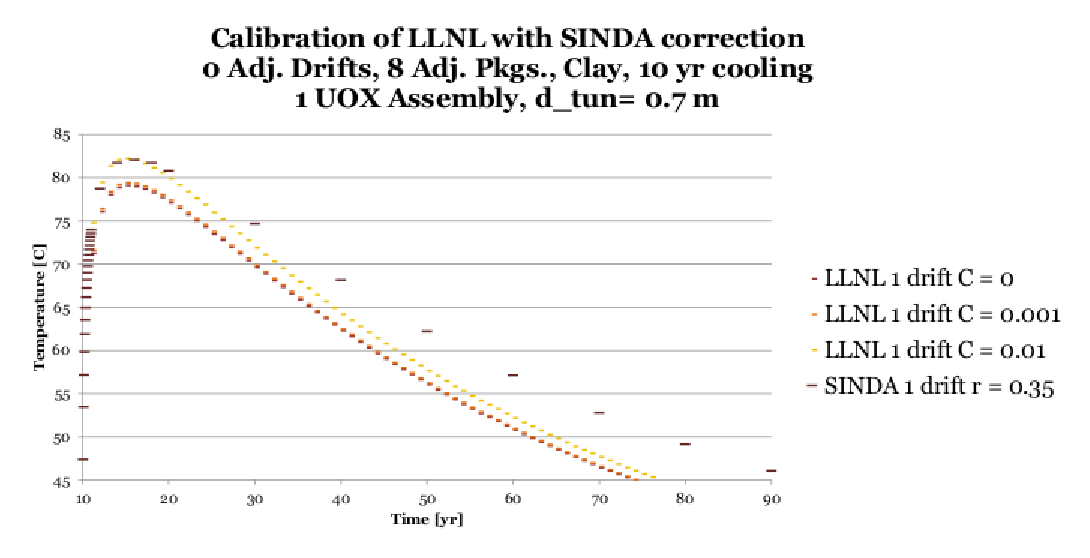
\includegraphics[width=0.8\textwidth]{1drift10yr.eps}
    \end{center}
    \caption{A single tunnel scenario was compared to the single tunnel repository 
    scenario run with the SINDA technique.}
    \label{fig:1drift10yr}
  \end{figure}
  
\end{frame}

\begin{frame}[ctb!]

  \frametitle{1 Tunnel 25 year}
  \begin{figure}[h!]
    \begin{center}
      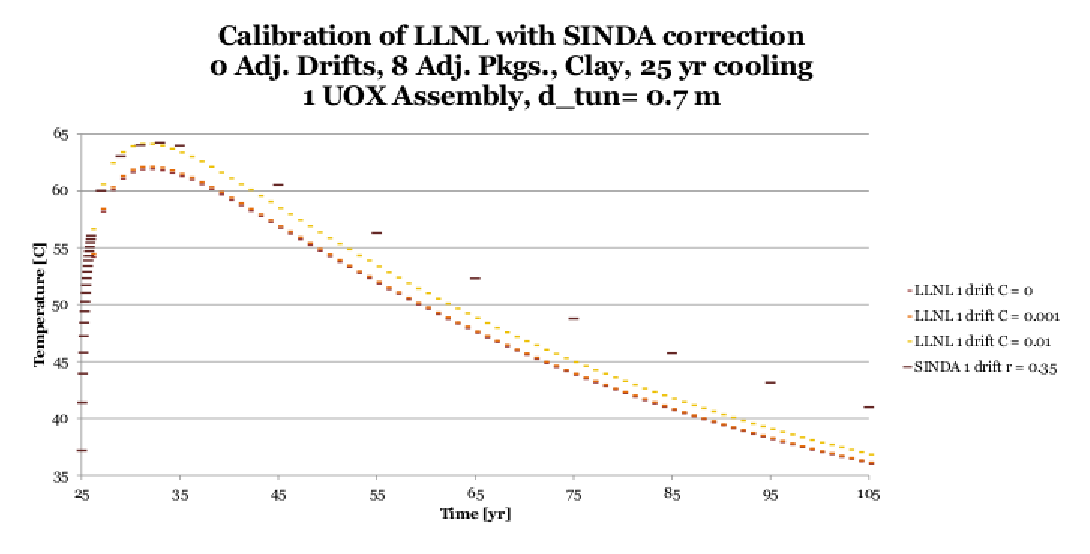
\includegraphics[width=0.8\textwidth]{1drift25yr.eps}
    \end{center}
    \caption{A single tunnel scenario was compared to the single tunnel repository 
    scenario run with the SINDA technique.}
    \label{fig:1drift10yr}
  \end{figure}
  
\end{frame}

\begin{frame}[ctb!]
  \frametitle{1 Tunnel 50 year}
  \begin{figure}[h!]
    \begin{center}
      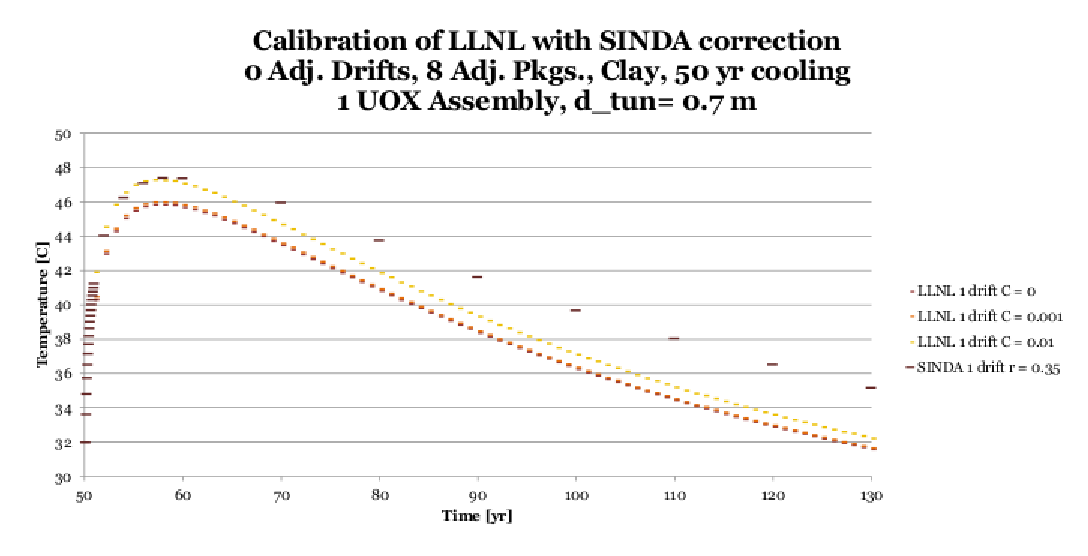
\includegraphics[width=0.8\textwidth]{1drift50yr.eps}
    \end{center}
    \caption{A single tunnel scenario was compared to the single tunnel repository 
    scenario run with the SINDA technique.}
    \label{fig:1drift50yr}
  \end{figure}
  
\end{frame}

